% !TEX root = main.tex

\documentclass[twocolumn]{article}

% Required packages
\usepackage{graphicx}  % For images
\usepackage{amsmath, amssymb} % Math symbols
\usepackage[external]{gnuplottex}
\usepackage{titlesec} % Formatting sections
\usepackage{fancyhdr} % Header and Footer customization
\usepackage{abstract} % Abstract formatting
\usepackage{titling} % Title customization
\usepackage{authblk} % Author affiliations
\usepackage{babel} % For figure legends
\usepackage{siunitx} % For SI units
\usepackage{hyperref} % For hyperlinks in the PDF
\usepackage{lipsum} 

\usepackage{blindtext} % Package to generate dummy text throughout this template 
\usepackage[sc]{mathpazo} % Use the Palatino font
\usepackage[T1]{fontenc} % Use 8-bit encoding that has 256 glyphs
\linespread{1.05} % Line spacing - Palatino needs more space between lines
\usepackage{microtype} % Slightly tweak font spacing for aesthetics
\usepackage{float}
\usepackage[a4paper, margin=1in,hmarginratio=1:1,top=15mm,left=12mm,bottom=25mm,columnsep=15pt]{geometry} % Document margins
\usepackage{enumitem} % Customized lists
\setlist[itemize]{noitemsep} % Make itemize lists more compact
\usepackage{abstract} % Allows abstract customization
\renewcommand{\abstractnamefont}{\normalfont\bfseries} % Set the "Abstract" text to bold
\renewcommand{\abstracttextfont}{\normalfont\small\itshape} % Set the abstract itself to small italic text
\usepackage{titlesec} % Allows customization of titles
\renewcommand\thesection{\Roman{section}} % Roman numerals for the sections
\renewcommand\thesubsection{\roman{subsection}} % roman numerals for subsections
\titleformat{\section}[block]{\large\scshape\centering}{\thesection.}{1em}{} % Change the look of the section titles
\titleformat{\subsection}[block]{\large}{\thesubsection.}{1em}{} % Change the look of the section titles


% Define Cover Page
\newcommand{\coverpage}{
    \begin{titlepage}
        \centering
        \vspace*{2cm}
        {\Huge \textbf{Quantum-inspired machine learning on a quantum computer}}\\[1cm]
        {\Large João Guilherme}\\[0.5cm]
        {\large Instituto Superior Técnico, Department of Physics}\\[2cm]
        {\large \today}\\[3cm]
        \vfill
        \begin{abstract}
            This document presents...
        \end{abstract}
        \vfill
    \end{titlepage}
}



\begin{document}

\coverpage

\section{Introduction}
Radial Basis Function (RBF) networks are a class of machine learning models well-suited for interpolation and classification tasks. Their foundation lies in constructing a hypothesis as a weighted sum of radial basis functions---functions whose output depends solely on the distance from a central point. This property allows RBF networks to capture local structures in the data efficiently.

This report details the construction and training of an RBF network applied to image classification, particularly using the MNIST dataset. We describe the mathematical formulation of the model, data encoding strategies including quantum-inspired Gram matrix encodings, and practical training methods including both full and reduced center approaches.

\section{Data Encoding}
\subsection{Gram Matrix Encoding}

We consider a column vector $u$ representing an image sample. To embed this into a higher-order representation, we construct the normalized outer product:
\[
\rho = \frac{uu^T}{\text{Tr}(uu^T)}
\]
This yields a density-like matrix $\rho$ with trace 1, encoding pairwise correlations between pixels. Such an encoding is inspired by quantum mechanical density operators and preserves structural information in the image.

\begin{figure}[h!]
    \centering
    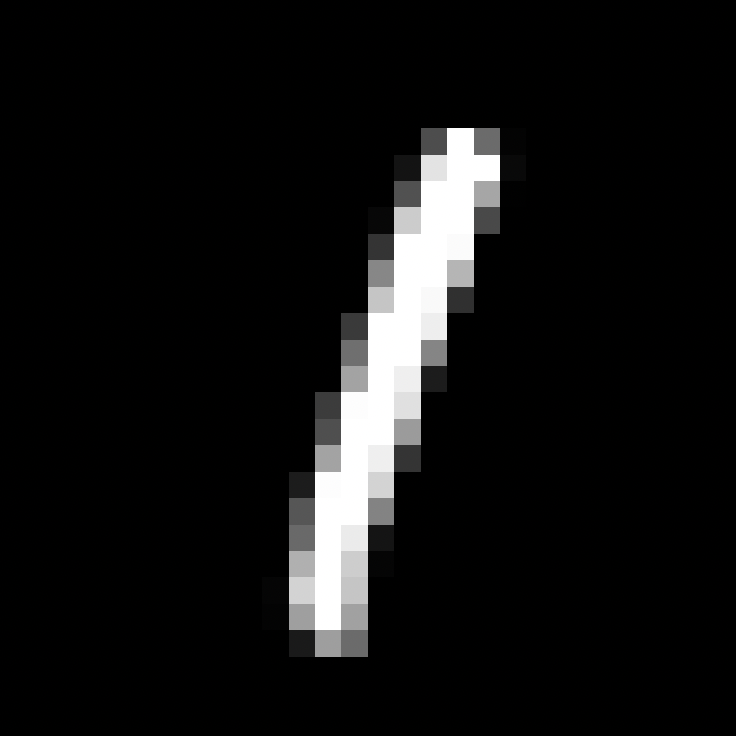
\includegraphics[width=0.6\linewidth]{figures/nmist_1_data.png}
    \caption{Example MNIST image (digit 1)}
    \label{fig:dataset_one}
\end{figure}

\begin{figure}[h!]
    \centering
    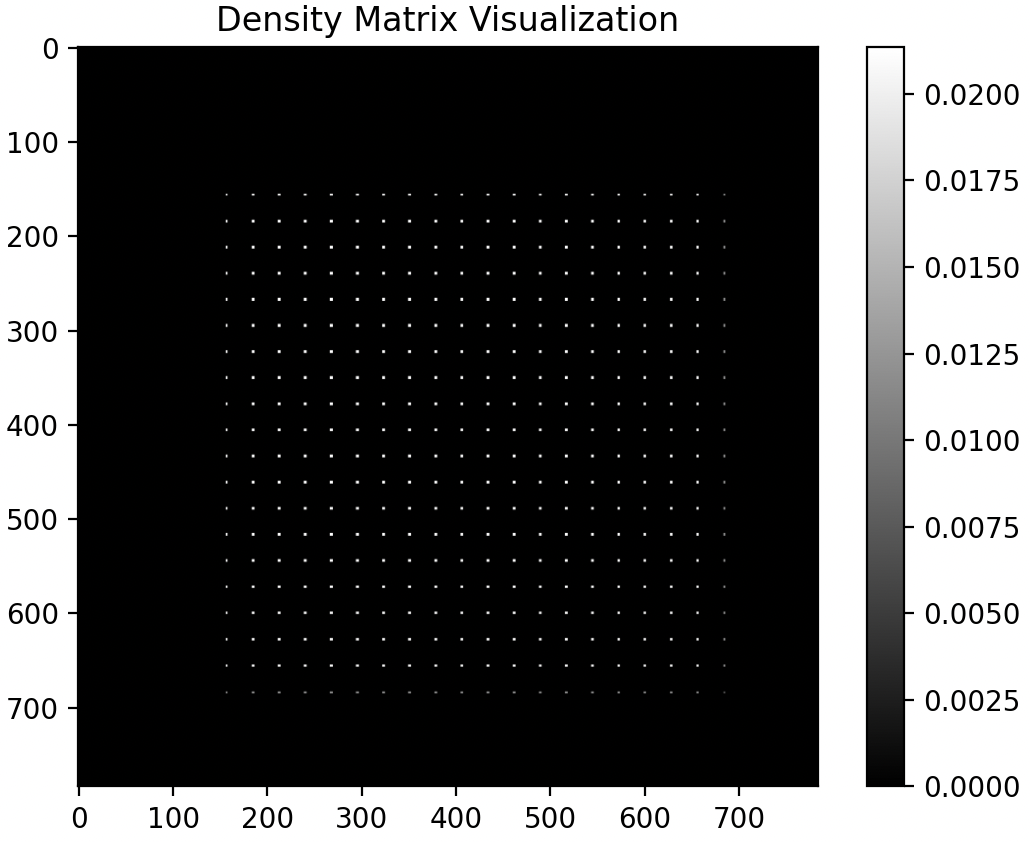
\includegraphics[width=0.6\linewidth]{figures/density_matrix_nmist_one.png}
    \caption{Gram matrix encoding $\rho$ of the digit 1 image}
    \label{fig:density_matrix}
\end{figure}

\section{Radial Basis Function Network}

RBF networks model the hypothesis function $h(x)$ using a radial function centered around key points (called \emph{centers}). Each center influences the prediction based on its proximity to the input $x$. The standard form is:
\[
h(x) = \sum_{n=1}^N w_n\exp\left(-\gamma\| x - x_n \|^2\right)
\]
where $\gamma$ determines the width of the radial functions, and $w_n$ are the learned weights.

\subsection{Exact Interpolation}
Given training data $D = \{(x_1, y_1), \dots, (x_N, y_N)\}$, we can formulate the interpolation condition:
\[
\sum_{m=1}^N w_m\exp\left(-\gamma\| x_n - x_m \|^2\right) = y_n, \quad \forall n
\]
In matrix notation:
\[
\Phi \mathbf{w} = \mathbf{y}, \quad \text{where } \Phi_{n,m} = \exp\left(-\gamma\|x_n - x_m\|^2\right)
\]
If $\Phi$ is invertible, we can directly solve:
\[
\mathbf{w} = \Phi^{-1} \mathbf{y}
\]
This yields an exact interpolating function.

\subsection{Classification}
For classification, we apply a decision rule such as:
\[
h(x) = \operatorname{sign}\left(\sum_{n=1}^N w_n\exp(-\gamma\|x - x_n\|^2)\right)
\]
In multi-class settings, this can be extended to a softmax output over class scores.

\subsection{Training with Least Squares}
Instead of enforcing exact interpolation, we may use a least squares approach to minimize:
\[
E = \sum_{n=1}^N (h(x_n) - y_n)^2
\]
This leads to the ridge-regularized solution:
\[
\mathbf{w} = (\Phi^T\Phi + \lambda I)^{-1}\Phi^T \mathbf{y}
\]
where $\lambda$ is a regularization parameter.

\section{Choosing RBF Centers}
Using every data point as a center is computationally expensive. Instead, we reduce the number of centers to $K \ll N$ by clustering the dataset using \textbf{K-Means}:

We define:
\[
J = \sum_{k=1}^K \sum_{x_n \in S_k} \| x_n - \mu_k \|^2
\]
and use Lloyd's algorithm to iteratively minimize $J$:
\begin{align*}
\mu_k &= \frac{1}{|S_k|}\sum_{x_n \in S_k} x_n \\
S_k &= \{ x_n : \|x_n - \mu_k\| \leq \|x_n - \mu_j\|,\ \forall j \neq k \}
\end{align*}

Repeat these steps until convergence. Since the process is sensitive to initialization, we typically run K-Means multiple times and choose the best clustering.

\begin{figure}[h!]
    \centering
    % Consider plotting a 3D Gaussian RBF here with Gnuplot
    \begin{gnuplot}[scale=0.6, terminal=pdf]
set title "3D Gaussian Function"
set xlabel "x"
set ylabel "y"
set zlabel "z"
set hidden3d
set view 60, 80
set isosamples 50, 50
set xrange [-5:5]
set yrange [-5:5]

# Parameters for the Gaussian
sigma = 1.0
mu_x = 0.0
mu_y = 0.0

# 2D Gaussian Function
gaussian(x, y) = exp(-((x - mu_x)**2 + (y - mu_y)**2) / (2 * sigma**2))

splot gaussian(x, y) with lines palette
\end{gnuplot}
    \caption{Example of a Gaussian RBF centered at $\mu$}
    \label{fig:gaussian_rbf}
\end{figure} 

\section{Implementation Notes}
The RBF network was implemented in Python using NumPy and scikit-learn. To avoid memory issues, we:
\begin{itemize}
    \item Use MiniBatchKMeans to find centers efficiently.
    \item Use perceptron-based or regularized least squares learning.
    \item Avoid computing large $\Phi^T\Phi$ matrices when possible.
\end{itemize}

\section{Conclusion}
RBF networks provide an elegant and powerful framework for classification. Through Gaussian kernel construction and data-driven center selection, they can adapt to local structures in the data. When combined with efficient encodings such as Gram matrices and practical training algorithms, they scale to real-world tasks like digit recognition.

\bibliography{references}{}
\bibliographystyle{plain}

\end{document}
